\section{An overview of $\Delta$QSD}
    $\Delta$QSD is defined as \cite{myo}:
    \begin{quote}
        ``A metrics-based, quality-centric paradigm that uses formalised outcome diagrams to explore the performance consequences of design decisions''.
    \end{quote}
    
    The key concepts that give the paradigm its name are \textbf{quality attenuation ($\Delta$Q)} and \textbf{outcome diagrams}. \cite{dq-tut}

    The dependency and causality properties of a system can be captured by outcome diagrams, while the probability distribution representation ($\Delta$Q) can precisely model a system's behaviour. \cite{myo}
 
    The following sections are a summary of multiple articles and presentations formalising the paradigm. Some of the graphs we present have too been adapted from the articles.
     
 \subsection{Outcome}
    To build outcome diagrams, we need to first introduce outcomes.

        Outcomes represent system behaviours or tasks that ``can start at some point in time and \textit{\textbf{may}} be observed to complete at some later time'' \cite{dq-br}.
        The result produced by performing a system's task is mapped to an outcome. \cite{myo} 
     
        The particularity of outcomes is that they can represent multiple levels of granularity. Suppose an outcome is beyond the current system's control (e.g. a database/cloud request), is non-atomic (can be broken down in multiple sub-outcomes). These outcomes can be represented as black boxes: you can observe their start and end, but do not know what is being executed. As the system gets refined, these outcomes can then be refined to model a single outcome or multiple outcomes, if needed. \cite{myo} \\ 
        Even though these outcomes are defined as ``black boxes'', they still have timeliness constraints like any other outcome. 

        Let us define some important concepts about outcomes.

     \paragraph{Observables}
     Key to outcomes is the notion of event. \\
     An outcome has observable starting events end ending events \cite{dq-tut}. As the events may occur in different locations in a distributed setting, we say the outcome has a starting set and ending set of events. They are called ``\textbf{observables}''. \cite{myo}\\
     We stated previously that an outcome \textbf{may} be observed to complete, this is because a starting event has no guarantee that it will be ended. An outcome can be said ``done'' if an end event occurs for a start event.

    \paragraph{Outcome instance}
    An outcome instance is the result of an execution of an outcome given a starting event $e_{in}$ and an end event $e_{out}$. \cite{art}

    \paragraph{Graphical Representation}
    Outcomes are represented as circles, with the starting and terminating set of events being represented by boxes. \cite{myo}
    \begin{figure}[H]
        \begin{center}
            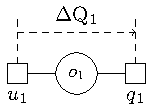
\includegraphics[scale=1.2]{tikz/outdq.pdf}
        \end{center}
        \caption{The outcome (circle) and the starting set (left) and terminating set (right) of events.}
    \end{figure}
   
  \subsection{Failure semantics} \label{subsec:failure}
       Failure indicates ``an input message $m_{in}$ \textbf{that has no output message} $m_{out}$'' \cite{art}. It models the probability that the delay is infinite.


\subsection{Quality attenuation ($\Delta$Q)}
    $\Delta$Q is defined as ``a cumulative distribution function (CDF) that defines both \textit{latency} and \textit{failure probability} between a start and end event''. \cite{dq-tut}
    
        As multiple instances of an outcome are executed, multiple delays can be observed for the executions. The observed delays can be represented as a CDF, we call it $\Delta$Q$_{obs}$. In the $\Delta$Q's CDF, \textbf{$\Delta$Q(x)} is the probability that an outcome $O$ occurs in time $t \le x$ \cite{art}.  We may sometimes use the derivative of a $\Delta$Q, which is the probability density function (PDF). We show a typical CDF of a $\Delta$Q in \cref{fig:int_mass}.

    The key feature that makes $\Delta$Q stands out is the notion of failure incorporated in the representation of an outcome's behaviour. \\
 Ideally, a system would execute without errors, failure or delay. This is never the case. Since the ideal cannot be attained, the quality of the system's responses are ``\textit{attenuated to the relative ideal}''  \cite{myo}. This quality attenuation gives the name to $\Delta$Q.

    Since multiple factors can influence the delays of a response (geographical, physical) \cite{dq-tut}, $\Delta$Q can be firstly modeled as a random variable. Nevertheless, as it incorporates failures, which are discrete variables, and delays, which are continuous random variables, the authors describe it as an \textit{Improper Random Variable}, as the probability of a finite or bounded delay is $<$ 1. \cite{myo}
   
    \paragraph{Intangible mass} Depicted in \cref{fig:int_mass}, the \textbf{\textit{intangible mass}} $1 - \lim_{x\to\infty}\Delta Q(x)$ of a $\Delta$Q encodes the probability of failure/timeout/exception occurring. \cite{art}\label{int_mass}
        
    \begin{figure}[H]
        \begin{center}
            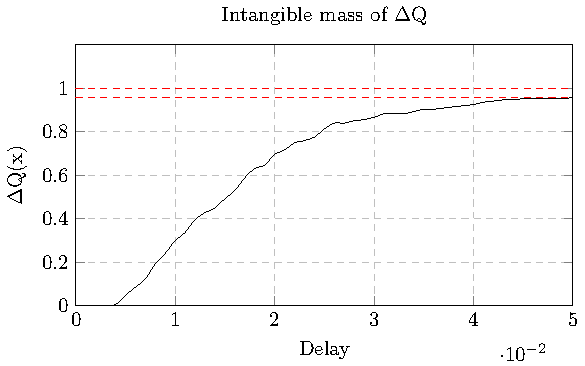
\includegraphics{tikz/intangible.pdf}
        \end{center}
        \caption{$\Delta$Q CDF representation with intangible mass (red, dotted). The failure rate is about 5\% }
        \label{fig:int_mass}
    \end{figure}

    \subsection{Partial ordering}
        We say $\Delta$Q$_1$ is \textit{less than} another $\Delta$Q$_2$ if its CDF is everywhere to the left and above the other's CDF. This concept is represented mathematically as a partial order. \cite{dq-tut} 

    \subsection{Timeliness}
        Timeliness is ``delivering results within required time bounds (sufficiently often)''. \cite{dq-tut}
       
    \subsection{QTA, required $\Delta$Q}
        The Quantitative Timeliness Agreement (QTA) specifies the precise timeliness requirements ($\Delta$Q$_{req}$) of a $\Delta$Q$_{obs}$. \cite{dq-br} \cite{art}

     Leveraging the definition of partial ordering and timeliness, we can say that a system \textit{satisfies timeliness} if $\Delta$Q$_{obs}$ $\le$ $\Delta$Q$_{req}$. \cite{art} 
    
    \paragraph{Slack and hazard} There is performance \textit{slack} when ``a $\Delta$Q is strictly less than the requirement.'' ($\Delta$Q$_{obs}$ < $\Delta$Q$_{req}$). \\
    There is performance \textit{hazard} when ``an observed $\Delta$Q$_{obs}$ intersects or is strictly greater than the required $\Delta$Q$_{req}$'' ($\Delta$Q$_{obs} \nless \Delta$Q$_{req}$). \cite{myo}
 
    \paragraph{QTA example} Imagine a system where 25\% of the executions should take $<$ 15 ms, 50\% $<$ 25 ms and 75\% $<$ 35 ms, all queries have a maximum delay of 50ms and 5\% of executions can timeout, the QTA can be represented as a step function. \\
    We present in \cref{fig:qta_step} an example of systems showing slack and hazard.
        \begin{figure}[H]
            \begin{center}
                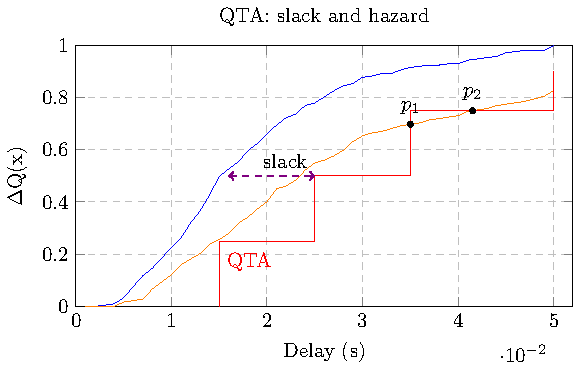
\includegraphics[scale=1.2]{tikz/cdf_qta_slack.pdf}
            \end{center}
            \caption{The system in blue (circle) is showing slack and satisfies the requirement. The system in orange (diamond) is showing signs that it cannot handle the stress, it is not respecting the system requirements imposed by the QTA. It intersects with the QTA in $p_1, p_2$, so it is not respecting the timeliness requirements. There is performance hazard.}%
            \label{fig:qta_step}
        \end{figure}

    \subsection{Outcome diagram}
        An outcome diagram is central to capture the causal relationships between the outcomes \cite{myo}. It shows the causal connections between all the outcomes we are interested in. Given an outcome diagram, one can compute the $\Delta$Q for the whole system. \\
        There are four different operators that represent the relationships between outcomes. \cite{dq-tut}
    \subsubsection{Sequential composition}
        If we assume two outcomes $O_A$, $O_B$ where the end event of $O_A$ is the start event of $O_B$, then we say the two outcomes are sequentially composed. The total delay $\Delta$Q$_{AB}$ is given by the convolution of the PDFs of $O_A$ and $O_B$ ($O_A \circledast O_B$). 
        \begin{figure}[H]
            \begin{center}
                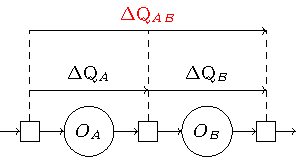
\includegraphics[scale=1]{tikz/seq_comp.pdf}
            \end{center}
            \caption{Sequential composition of $O_A$ and $O_B$.}
        \end{figure}
        Where convolution ($\circledast$) between two PDF is:
        \begin{equation}
            PDF_A \circledast PDF_B (t) = PDF_{AB}(t) =\int\limits_0^t PDF_A(\delta) \cdot PDF_B(t-\delta) \  d\delta 
            \label{eq:conv_1}
        \end{equation}

        Thus, $\Delta$Q$_{AB}$:
        \begin{equation}
            \Delta Q_{AB} = \int_0^t PDF_{A} \circledast PDF_{B} \ d\delta
            \label{eq:convolution_pdf}
        \end{equation}

        Convolution is the only operation which is based on the PDFs, the following operations are based on the CDF of the $\Delta$Qs (hence the use of the $\Delta$Q notation).
        
    \subsubsection{First to finish (FTF)}
            If we assume two independent outcomes $O_A$, $O_B$ with the same start event, first-to-finish occurs when at least one end event occurs, it can be calculated as:
        \begin{equation}
            \begin{split}
                (1 - \Delta Q_{FTF(A, B)}) &= Pr[d_A > t \wedge d_B > t] \\
                & = Pr[d_A > t] \cdot Pr[d_B > t] = (1 - \Delta Q_A) \cdot (1 - \Delta Q_B) \\
                \Delta Q_{FTF(A, B)} &= \Delta Q_A + \Delta Q_B - \Delta Q_A \cdot \Delta Q_B  
            \end{split}    
            \label{eq:ftf} 
        \end{equation}

       \begin{figure}[H]
            \centering
            \begin{subfigure}{.5\textwidth}
                \centering
                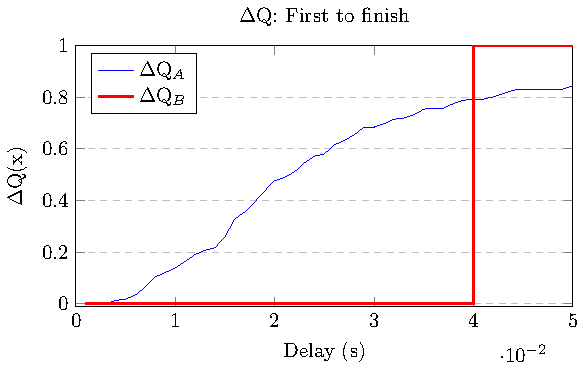
\includegraphics[scale = 0.7]{tikz/ftf_1.pdf}
                \label{fig:ftf1}
            \end{subfigure}%
            \begin{subfigure}{.5\textwidth}
                \centering
                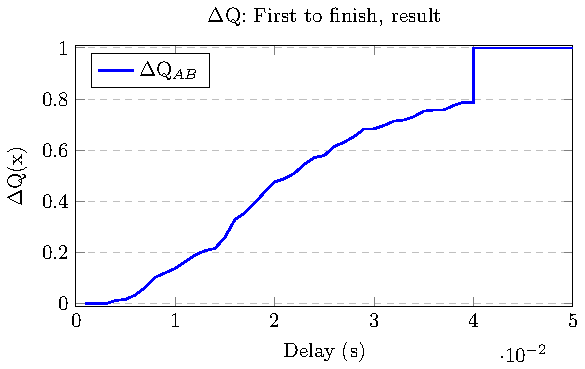
\includegraphics[scale = 0.7]{tikz/ftf_2.pdf}
                \label{fig:ftf2}
            \end{subfigure}
            \caption{Left: $\Delta$Q$_{(A, B)}$. Right: FTF$_{(A, B)}$ = $\Delta$Q$_{AB}$}%
            \label{fig:ftf}
            \end{figure}

    \subsubsection{All to finish (ATF)}
        If we assume two independent outcomes $O_A$, $O_B$ with the same start event, all-to-finish occurs when both end events occur, it can be calculated as:
        \begin{equation}
            \begin{split}
                \Delta Q_{ATF(A, B)} &= Pr[d_A \le t \wedge d_B \le t] \\
                & = Pr[d_A \le t] \cdot Pr[d_B \le t] = \Delta Q_A \cdot \Delta Q_B \\
                \Delta Q_{ATF(A, B)} &= \Delta Q_A \cdot \Delta Q_B 
            \end{split}
            \label{eq:atf}
        \end{equation}
        
        \begin{figure}[H]
            \centering
            \begin{subfigure}{.5\textwidth}
                \centering
                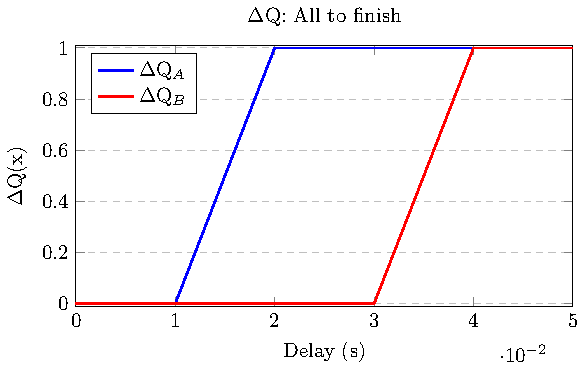
\includegraphics[scale = 0.7]{tikz/atf_1.pdf}
                \label{fig:atf_1}
            \end{subfigure}%
            \begin{subfigure}{.5\textwidth}
                \centering
                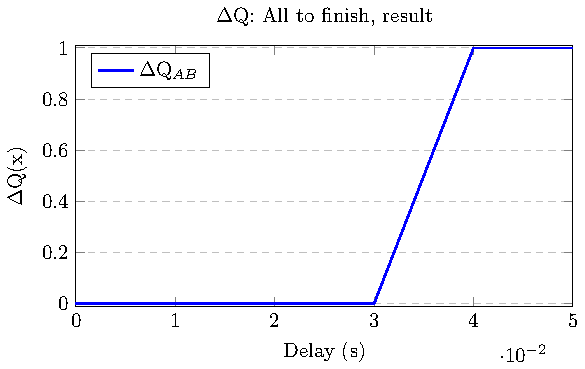
\includegraphics[scale = 0.7]{tikz/atf_2.pdf}
                \label{fig:atf2}
            \end{subfigure}
            \caption{Left: $\Delta$Q$_{(A, B)}$. Right: ATF$_{(A, B)}$ = $\Delta$Q$_{AB}$}%
            \label{fig:atf}
            \end{figure}

    \subsubsection{Probabilistic choice (PC)}
        If we assume two possible outcomes $O_A$ and $O_B$ and exactly one outcome is chosen during each occurrence of a start event and:
        \begin{itemize}
            \item $O_A$ happens with probability $\dfrac{p}{p+q}$
            \item $O_B$ happens with probability $\dfrac{q}{p + q}$
        \end{itemize}
        \begin{equation}
           \Delta Q_{PC}(A, B) = \dfrac{p}{p + q}\Delta Q_A + \dfrac{q}{p + q}\Delta Q_B 
            \label{eq:pc}
        \end{equation} 

    \begin{figure}[H]
        \begin{center}
            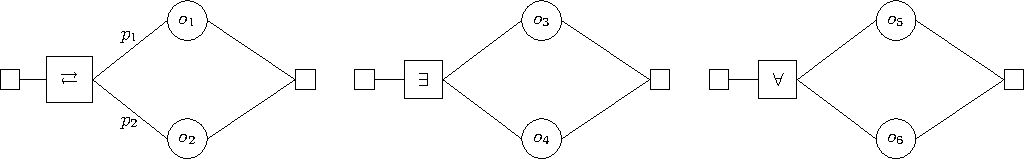
\includegraphics[width = \textwidth]{tikz/op.pdf}
        \end{center}
        \caption{Graphical representation of the possible operators in an outcome diagram. From left to right: Probabilistic choice, first-to-finish, all-to-finish. \cite{myo}}
        \label{fig:op}
    \end{figure}
    First-to-finish, All-to-finish and probabilistic-choice are calculated on the CDF of the $\Delta$Qs of their components.
    
    These operators can be assembled together to create an outcome diagram. In Chapter 4 we will see how one can go from the graphical representation to outcome diagrams which can be used in the $\Delta$Q oscilloscope.
    
    \subsection{Outcome diagrams refinement}
        An important feature of outcome diagrams is the ability to be able to design a system even with \textit{``black boxes''}, before the complete details of it are known. \cite{myo} \\
        An outcome diagram can be ``unboxed'' by refining the outcomes that compose it. We can adapt a situation described by the previously cited article, called ``Mind your Outcomes'', to understand how refinement can allow the user to have a very precise representation of a system. 
        
        We first start with a black box, unnamed outcome with start event $A$ and end event $Z$, somewhere in the system. The first refinement step would be giving the outcome a name.

      \begin{figure}[H]
            \begin{center}
                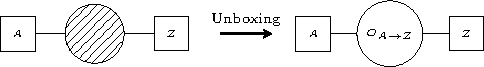
\includegraphics[scale = 1]{tikz/black_box.pdf}
            \end{center}
            \caption{Refinement from black box to named outcome.}
            \label{fig:bb}
        \end{figure}

    The system can be further refined by adding outcomes that represent tasks. For example, the engineer might believe that it will take two tasks to get from A to Z. We can then add another outcome, sequentially composed, to represent this situation.

       \begin{figure}[H]
            \begin{center}
                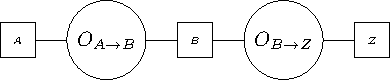
\includegraphics[scale = 1]{tikz/out_2.pdf}
            \end{center}
            \caption{Further refinement from one task to two tasks.}
            \label{fig:2_hops}
        \end{figure}

        We can also model the chance of executing two tasks as a probabilistic choice, where there is $p_2$ probability that the execution from A to Z will execute two tasks. The outcome diagram can be refined as a probabilistic choice.

   \begin{figure}[H]
            \begin{center}
                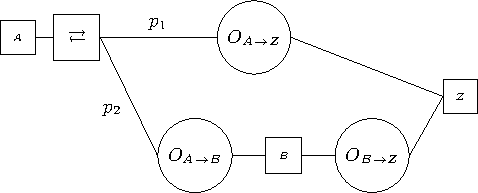
\includegraphics[scale = 1]{tikz/ref_op.pdf}
            \end{center}
            \caption{Refinement as probabilistic choice of executing either one or two tasks.}
            \label{fig:prob_ref}
        \end{figure}
    In essence, the refinement could model a very fine-grained representation of the system by further refining the system, to represent the possibility of executing $n$ tasks. This demonstrates the power of outcome diagrams to represent system diagrams with high precision. They can help explore design decisions thanks to outcomes and operators.

    \subsection{Independence hypothesis} \label{indep_hyp} 
        An important aspect of sequential composition is the assumption of outcomes having independent behaviour \cite{post}. Let us explain the following assumption clearly.

        Assume the situation described by \cref{fig:otc_indep}, two sequentially composed outcomes $o_1$, $o_2$ running on the same processor. The overall delay of execution can be observed from the start event of $o_1$ ($u_1$) to the end event of $o_2$ ($r_1$). 
        \begin{figure}[H]
            \begin{center}
                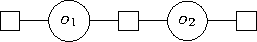
\includegraphics[scale=1]{tikz/indep.pdf}
            \end{center}
            \caption{Two sequentially composed outcomes, $o_1$, $o_2$. The end event of $o_1$ is the start event of $o_2$.}%
            \label{fig:otc_indep}
        \end{figure} 
        At low load, the two components behaviour will be independent (\cref{fig:cdf_indep}), the system will behave \textbf{linearly}. According to the superposition principle, the overall delay will be the sum of the two delays, as will the overall processor utilisation. \cite{sup-p}
        
        When load increases, the two components will start to show dependent behaviour due to the processor utilisation increasing. The $\Delta$Q of the observed total delay will then deviate from the sum of the two delays ($o_1 \circledast o_2$). This situation is observed in \cref{fig:cdf_indep}.
        
        \begin{figure}[H]
            \begin{center}
                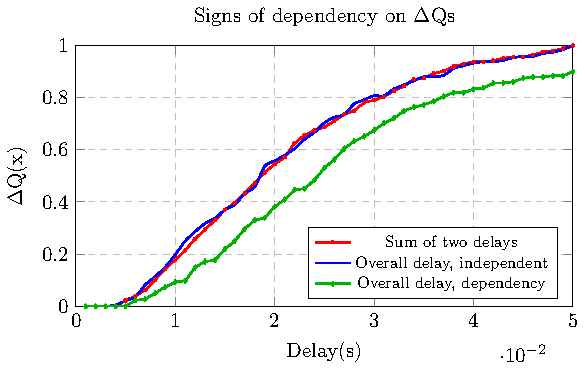
\includegraphics[scale=1]{tikz/cdf_indep.pdf}
            \end{center}
            \caption{When the components are independent, the sum of the two delays (blue) and the overall delay (red) can be superposed. As $o_1$ and $o_2$ show signs of dependency, the overall delay (green) can be seen deviating from the sum of the two delays. There is \textbf{non-linearity}.}
            \label{fig:cdf_indep}%
        \end{figure}%

        When the system is far from being overloaded, the effect is noticeable. As the cliff edge of overload is approached, the non-linearity will increase \cite{dq-tut} \cite{post}. These theoretical results can be observed in the oscilloscope. We will explore such cases in Chapter 6.
